\documentclass[a4paper,10pt]{book}
\usepackage[utf8x]{inputenc}
\usepackage{graphicx}
\DeclareGraphicsRule{.eps}{eps}{}{}
\usepackage{hyperref}

\title{Trasduttori}
\author{Federico Vaga}
\date{Giugno 2012}

\begin{document}
% stampa la licenza CC BY-NC-SA_2.5_IT
% occorre che i documento originale usi il pacchetto hyperref

\begin{center}\textbf{{\large Licenza - License}}\end{center}

\begin{figure}[hcbp]  
  \centering
  
\includegraphics{licenza/CreativeCommons/BY-NC-SA_2.5_IT/cc.png}
\end{figure}

\begin{center}\textbf{Italiano}\end{center}
“Questo lavoro è licenziato sotto licenza Creative Commons - Non commerciale - Condividi allo stesso modo 2.5 Italia (CC BY-NC-SA 2.5). Per vedere una copia di questa licenza visita il sito \url{http://creativecommons.org/licenses/by-nc-sa/2.5/it/}; oppure invia una lettera a Creative Commons, 171 2nd Street, Suite 300, San Francisco, California, 94105, USA.”\newline
\begin{center}\textbf{English}\end{center}
“This work is licensed under the Creative Commons Attribuzione - Non commerciale - Condividi allo stesso modo 2.5 Italia (CC BY-NC-SA 2.5) License. To view a copy of this license, visit \url{http://creativecommons.org/licenses/by-nc-sa/2.5/it/}; or, (b) send a letter to Creative Commons, 171 2nd Street, Suite 300, San Francisco, California, 94105, USA.” \newline



\tableofcontents
\listoffigures

\part{Trasduttori e attuatori}
\chapter{Introduzione}
Lo scopo di un trasduttore è quello di trasformare un segnale di
natura fisica in un segnale elettrico; per fare questo i trasduttori
si basano su principi fisici.
Per descrivere le caratteristiche di un trasduttore possiamo
catalogarle in statiche (cioè proprie del trasduttore) e dinamiche
(cioè che dipendono dal processo al quale lo si applica).
Fra le caratteristiche statiche abbiamo:
\begin{itemize}
 \item \textit{Sensibilità}: rapporto fra la variazione di grandezza
elettrica e di grandezza fisica.
	\[ \frac{\Delta GE}{\Delta GF} \]
 \item \textit{Risoluzione}: cioè la minima variazione valutabile
della grandezza fisica. Di conseguenza avremo una rappresentazione
della grandezza fisica con un segnale a gradini. Questa è la diretta
conseguenza del passaggio dallo spazio continuo (analogico/fisico)
allo spazio discreto (digitale).
 \item \textit{Soglia}: il minimo valore della grandezza fisica
misurabile.
 \item \textit{Range}: intervallo di valori della grandezza fisica in
esame che il trasduttore può misurare.
 \item \textit{Isteresi}: massima differenza tra due cammini di
andata e di ritorno dell'uscita del trasduttore durante un ciclo che
raggiunge gli estremi del range.
 \item \textit{condizioni ambientali}: condizioni ambientali che
garantiscono il corretto funzionamento; se il trasduttore viene fatto
lavorare fuori dalle condizioni nominali si possono generare errori.
 \item \textit{errore}: differenza fra il comportamento reale e
quello ideale, a questo viene anche associata una
 \item \textit{banda d'errore}: è una regione in cui i valori reali
possono differire da quelli ideali.
\end{itemize}

Le caratteristiche dinamiche di un trasduttore dipendono dal
funzionamento del processo al quale viene applicato, il problema
principale è verificare se il trasduttore scelto è in grado di seguire
fedelmente le variazioni del processo; per capirlo vengono forniti i
diagrammi di Bode della sensibilità del trasduttore (fig. d) e nel
caso in cui il trasduttore non riesca ad operare a frequenze troppo
basse viene fornita la banda di applicabilità (fig. e). Altra
caratteristica dinamica importante è l'affidabilità del trasduttore,
cioè la capacità di sopportare sovraccarichi, la vita media del
trasduttore.
\chapter{Trasduttori di posizione lineare}
\section{Potenziometro a filo avvolto}\label{sec:filoavvolto}
Si tratta di un filo di lega metallica con resistività e dimensioni
stabili che viene avvolto lungo un cilindro rigido; un cursore,
anch'esso metallico, viene poso sopra al cilindro di modo che possa
fare contatto sul filo avvolto e sarà proprio su questo cursore che
verrà prelevata la tensione di riferimento per il campionamento. In
figura \ref{fig:filoavvolto} è possibile vederne una
rappresentazione schematica, mentre in figura \ref{fig:potenziometro}
la rappresentazione circuitale.

\begin{figure}[htbp]
	\centering
	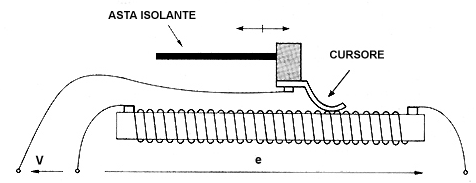
\includegraphics[scale=0.5]{img/filoavvolto.png}
	\caption{Potenziometro a filo avvolto\label{fig:filoavvolto}}
\end{figure}

\begin{figure}[htbp]
	\centering
	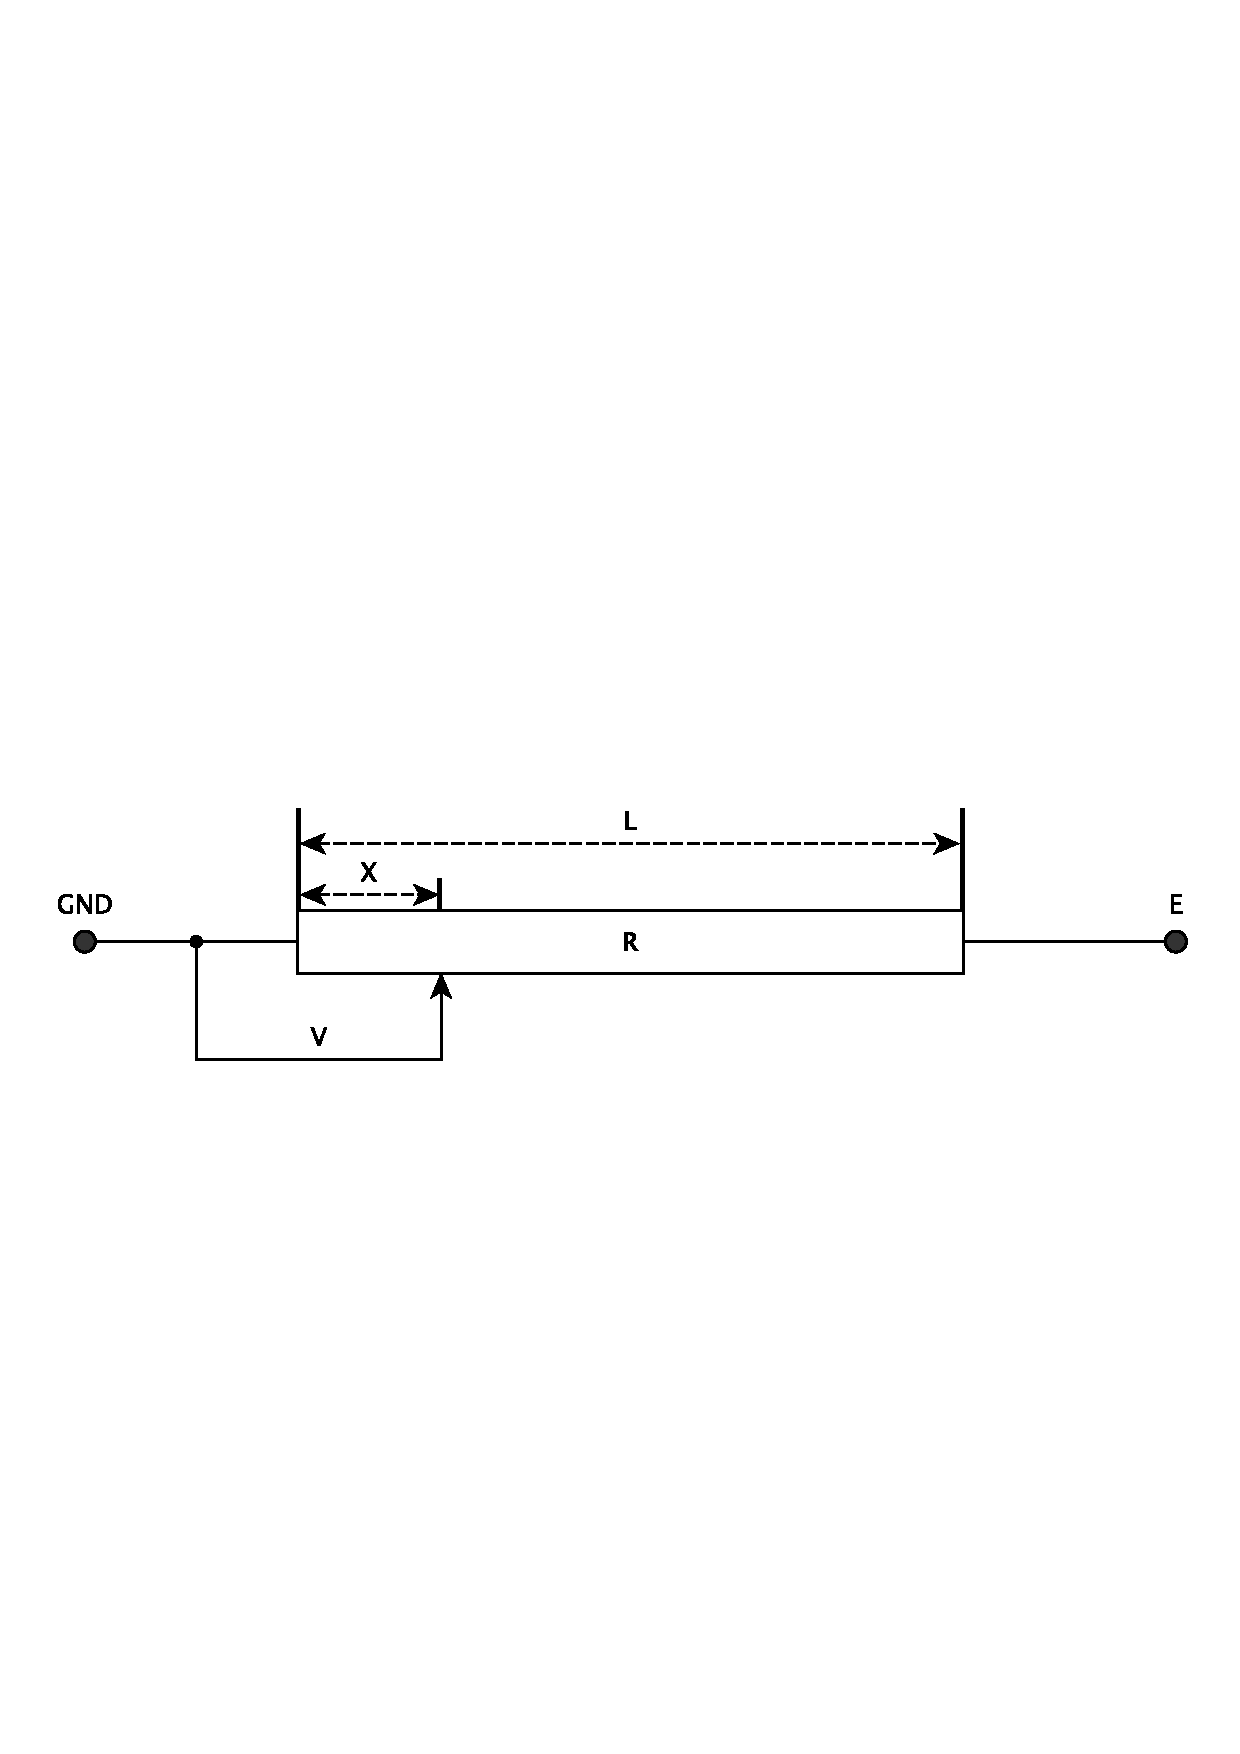
\includegraphics[scale=0.5]{img/potenziometro.pdf}
	\caption{Potenziometro\label{fig:potenziometro}}
\end{figure}

Per ricavare il valore della tensione in uscita V basta applicare la
regola del partitore di tensione, immaginando che le due resistenze
siano rappresentate: una dalla parte alla sinistra del cursore (sulla
quale si preleva la misura della tensione) e l'altra dalla parte alla
destra del cursore come in figura \ref{fig:potenziometroequiv}.

\begin{figure}[htbp]
	\centering
	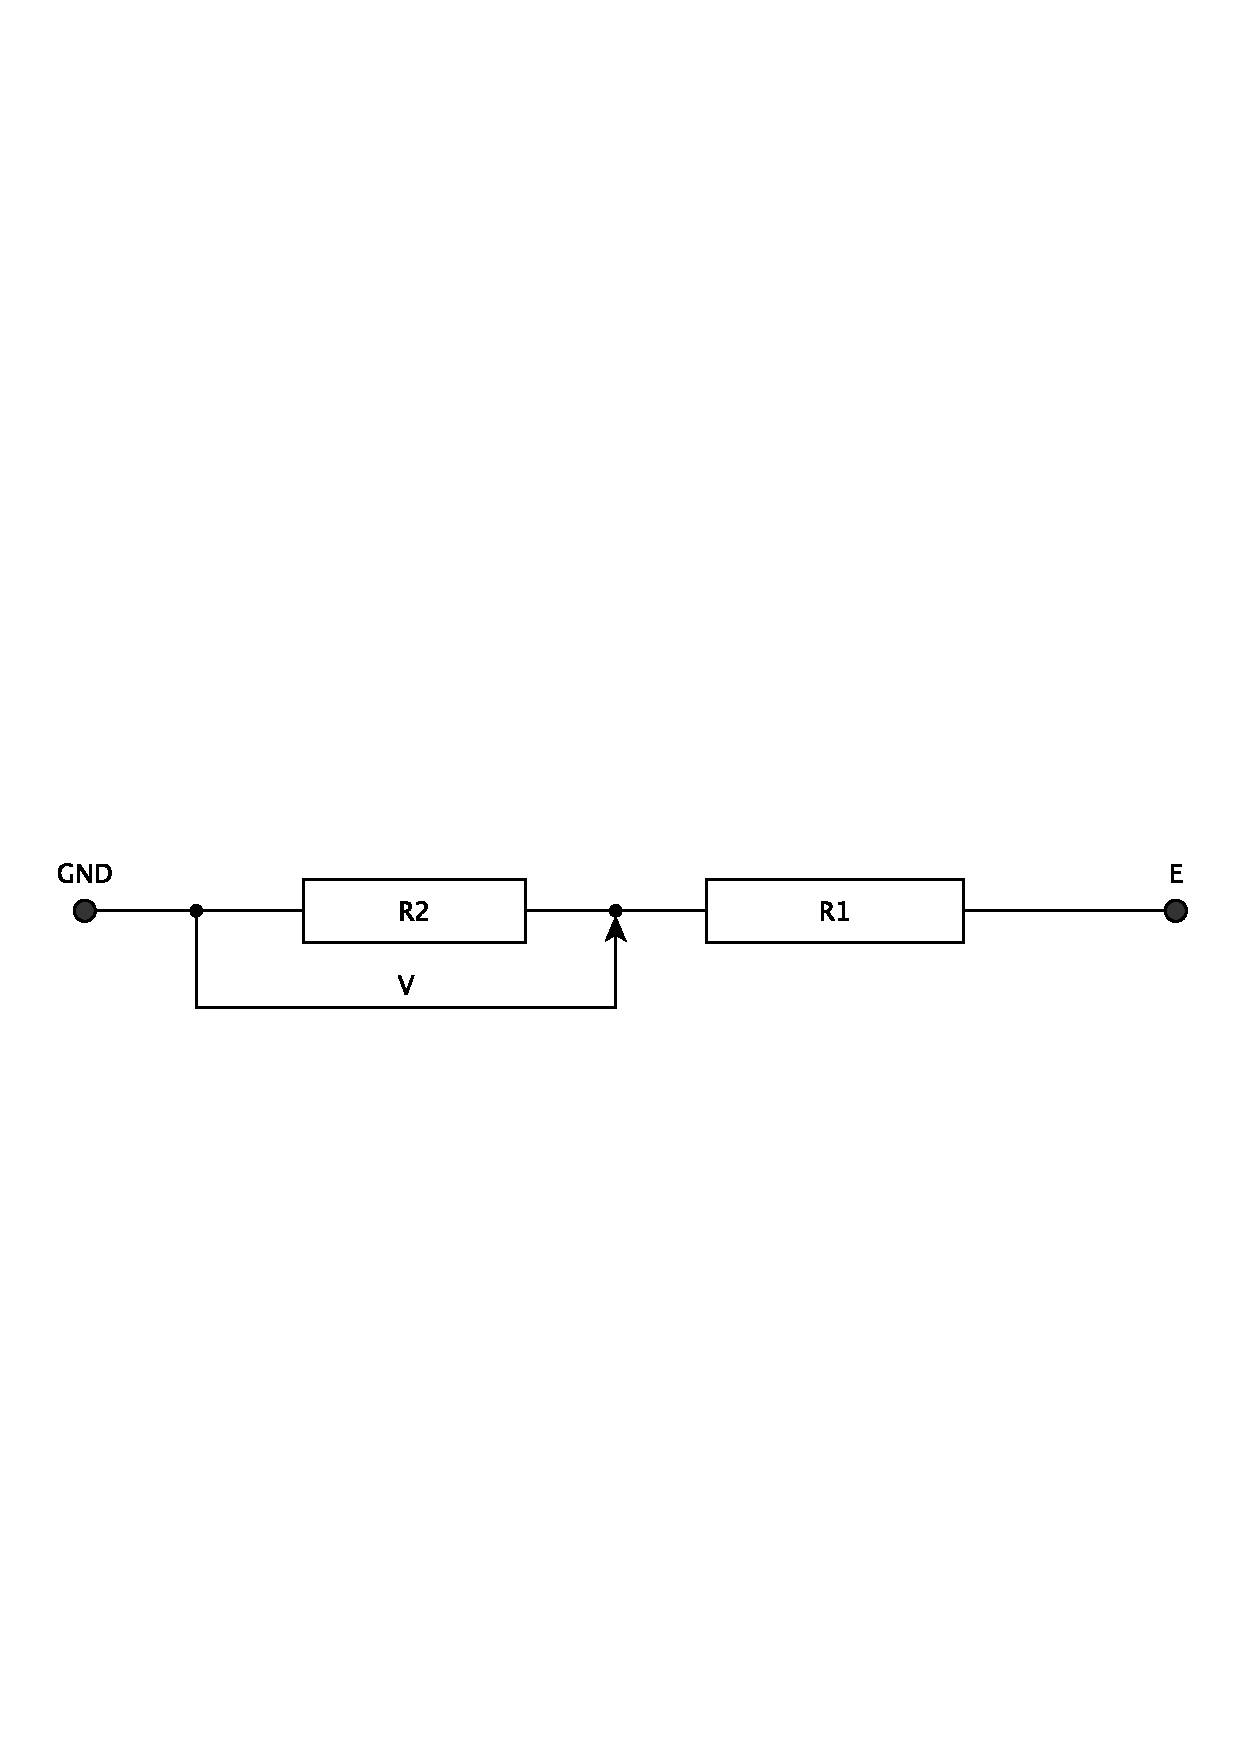
\includegraphics[scale=0.5]{img/potenziometro-equiv.pdf}
	\caption{Circuito equivalente
per il potenziometro\label{fig:potenziometroequiv}}
\end{figure}

Il problema è ora quantificare il valore di queste
due resistenze e metterlo in relazione con con lo spostamento $X$ del
cursore rispetto all'inizio (cioè quando il cursore è tutto a
sinistra). Ora indichiamo con $L$ la lunghezza del potenziometro e
calcoliamo $V$:

\[ R = \frac{L}{S}\rho \rightarrow R_1=\frac{L-S}{S}\rho,
R_2=\frac{S}{S}\rho \]
\[V=E\frac{R_2}{R_1+R_2}=E\frac{\rho\frac{X}{S}}{\rho\frac{L-X}{S}
+ \rho\frac{X}{S}}= E \frac{X}{L}\]

Da qui la relazione che lega $V$ con $X$:

	\[\frac{X}{L} = \frac{V}{E}\]

\subsection{Vantaggi}
Il primo vantaggio è la linearità: la resistività uniforme del cavo
permette una distribuzione di potenziale che è lineare nello spazio.
Un secondo vantaggio, è la possibilità di ottenere un segnale
elettrico di ampiezza desiderato. Il trasduttore è insensibile alla
variazione di temperatura se questa avviene uniformemente su l'intero
trasduttore.
\subsection{Svantaggi}
La risoluzione limitata dovuto allo spazio vuoto fra due avvolgimenti
del filo metallico, inoltre in questo spazio si può perdere la misura.
La vita media breve a causa dell'usura generata dal movimento del
cursore e, infine, la forza necessaria per vincere l'attrito generato
dal movimento del contatto provoca un'alterazione del sistema sotto
misura, quindi possono esserci possibili isteresi.

\section{Potenziometro a strato di carbonio}\label{sec:potcarbonio}
Il funzionamento è del tutto analogo a quello del potenziometro a filo
avvolto\ref{sec:filoavvolto} con la differenza che a fornire la
resistenza c'è ora uno strato di carbonio sul quale va a posizionarsi
il cursore.

\begin{figure}[htbp]
	\centering
	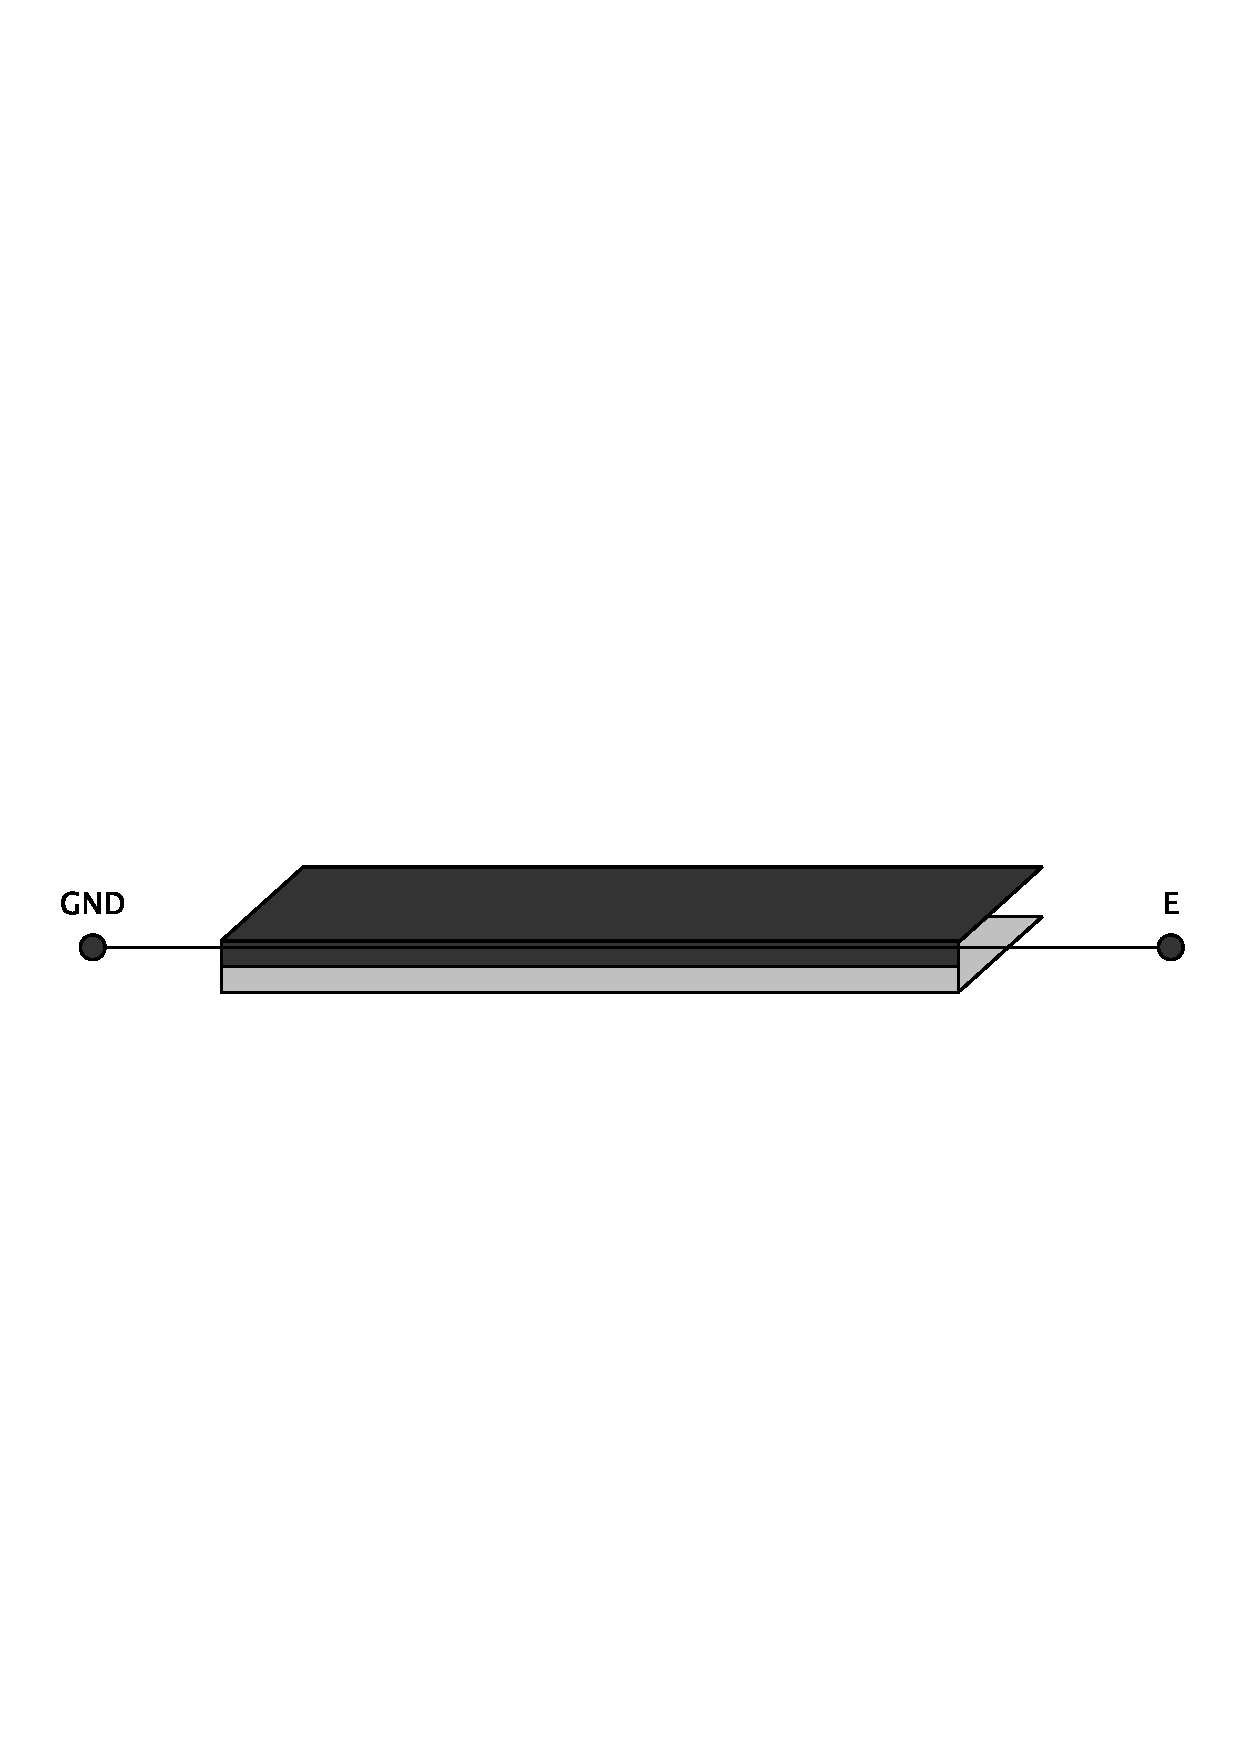
\includegraphics[scale=0.5]{img/potenziometro-carbonio.pdf}
	\caption{Potenziometro a
strato di carbonio\label{fig:potenziometro-carbonio}}
\end{figure}

Il vantaggio introdotto è che ora la risoluzione non è più
a scalino ma è lineare lontano dagli estremi, lo svantaggio invece è
la vita molto breve dovuto al consumo dello strato di carbonio causato
dallo sfregamento del cursore su di esso.

\section{Potenziometro elettro-ottico
(fotopotenziometro)}\label{sec:elettrottico}
Essendo un potenziometro, il suo comportamento è analogo a quello
visto per il potenziometro a filo avvolto\ref{sec:filoavvolto}, cambia
solo il modo in cui viene realizzato. La realizzazione di un
potenziometro elettro-ottico prevede di unire un film resistivo con
una striscia di materiale foto-conduttore e del materiale conduttore.

\begin{figure}[htbp]
	\centering
	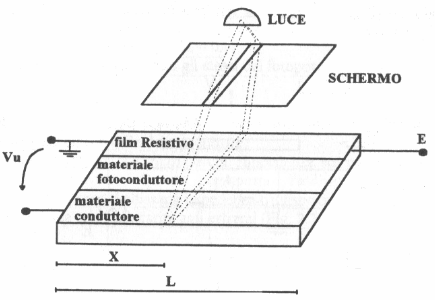
\includegraphics[scale=0.5]{img/fotopotenziometro.png}
	\caption{Foto-potenziometro\label{fig:fotopotenziometro}}
\end{figure}

A questo punto sopra a questi tre elementi viene posta una lamina
tagliata. Attraverso la lamina viene fatta passare la luce che farà
passare la corrente nel punto in cui il materiale fotoconduttore è
illuminato permettendo così di prelevare la tensione V sul materiale
conduttore.

\subsection{Vantaggi}
Il principale vantaggio è l'assenza di contati meccanici striscianti
e di conseguenza una vita più lunga del trasduttore. Questo tipo di
potenziometro offre una maggiore risoluzione.
\subsection{Svantaggi}
Questo tipo di potenziometro garantisce una linearità inferiore,
inoltre è molto più complesso, quindi costoso, da realizzare.
Richiede il buio totale in quanto le infiltrazioni di luce esterna
potrebbero introdurre errori.

\section{Trasduttore capacitivo}\label{sec:potcapacitivo}
Esso è costituito da tre armature di metallo di cui due fisse ed
allineate e una mobile che si muove sopra le altre due creando così
due capacità differenti che variano a seconda dell'area dell'armatura
mobile che copre una delle due armature. In figura
\ref{fig:potcapacitivo} una rappresentazione schematica.

\begin{figure}[htbp]
	\centering
	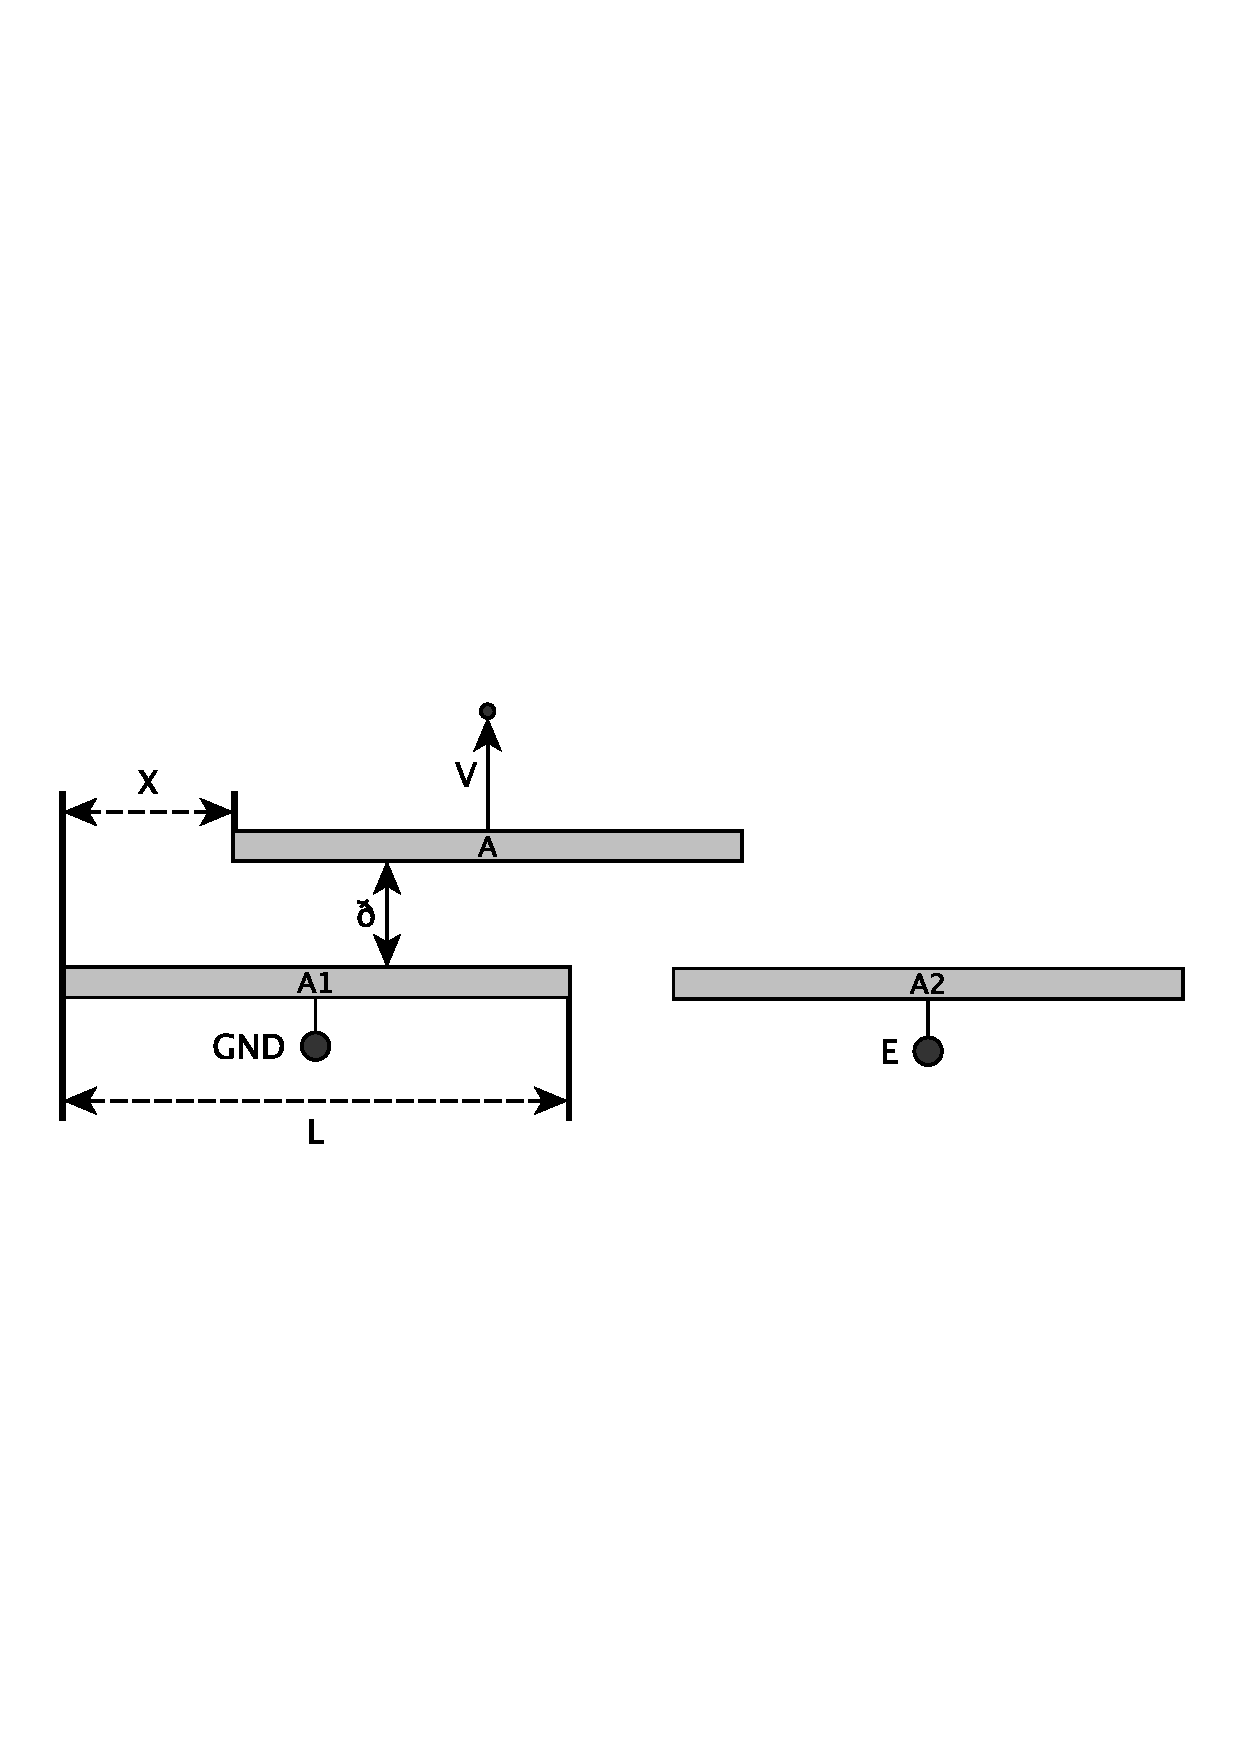
\includegraphics[scale=0.5]{img/potenziometro-capacitivo.pdf}
	\caption{Potenziometro capacitivo\label{fig:potcapacitivo}}
\end{figure}

In questo modo sempre col partitore di tensione possiamo misurare lo
spostamento. In figura \ref{fig:potcapacitivoequiv} il circuito
equivalente.

\begin{figure}[htbp]
	\centering
	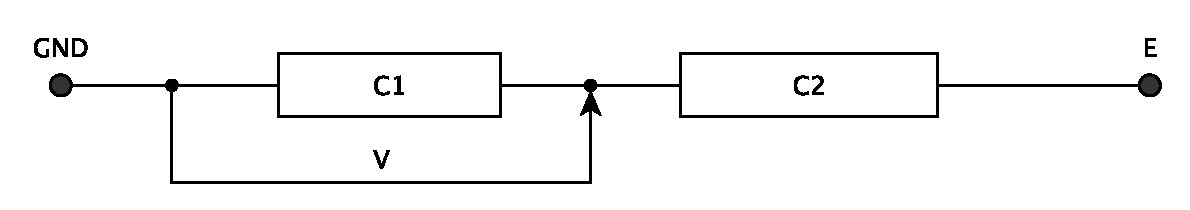
\includegraphics[scale=0.5]
{img/potenziometro-capacitivo-equiv.pdf}
	\caption{Circuito equivalente
del trasduttore capacitivo\label{fig:potcapacitivoequiv}}
\end{figure}

Le capacità $C_1$ e $C_2$ sono le capacità che si vengono a creare
dalla sovrapposizione delle armature $A_1$ e $A_2$ con l'armatura $A$.
$H$ indica la profondità dell'armatura.

	\[
	C_1=\frac{H (L-x)}{\delta}\varepsilon_0,
	C_2 =\frac{Hx}{\delta}\varepsilon_0
	\]
	\[
	V=E\frac{\frac{1}{sC_1}}{\frac{1}{sC_1}+\frac{1}{sC_2}}
	 =E\frac{C_2}{C_1+C_2}
	 =E\frac{\frac{Hx}{\delta}\varepsilon_0}
		{\frac{Hx}{\delta}\varepsilon_0+
				\frac{H(L-x)}{\delta}\varepsilon_0}
	 =E\frac{x}{L}
	\]

\subsection{Vantaggi}
I vantaggi sono gli stessi del potenziometro
elettro-ottico\ref{sec:elettrottico}
\subsection{Svantaggi}
Questo trasduttore soffre di scarsa linearità agli estremi; inoltre
si hanno problemi di carico inquanto l'impedenza del condensatore è
elevata, questo suggerisce l'utilizzo di un buffer ad alta
impedenza d'ingresso. Per ultimo, quando si lavora in
tensione alternata si rende necessario un circuito raddrizzatore a
valle del potenziometro.

\subsection{Variazione di impedenza}
Un alternativa è quella di usare un trasduttore di posizione
capacitivo a variazione d'impedenza, costruito come due cilindri che
si inseriscono uno dentro l'altro e muovendoli varia la capacità come
$C=KX$ e quindi anche l'impedenza.

\begin{figure}[htbp]
	\centering
	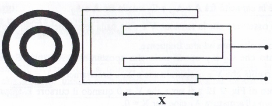
\includegraphics[scale=0.5]
{img/potenziometro-capacitivo-2.png}
	\caption{Potenziometro
capacitivo alternativo\label{fig:potcapacitivoalt}}
\end{figure}

\section{Trasformatore differenziale}
La trasduzione si basa sul principio della mutua induttanza variabile:
per realizzare ciò si utilizza un avvolgimento primario e due
avvolgimenti secondari di accoppiamento. L'accoppiamento avviene
tramite un cilindro ferromagnetico di sezione $S$ e lunghezza $L$ che
si muove fra il primario e il secondario.

\begin{figure}[htbp]
	\centering
	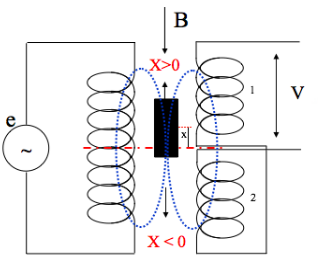
\includegraphics[scale=0.5]
{img/trasformatore-differenziale.png}
	\caption{Trasformatore differenziale\label{fig:trasdiff}}
\end{figure}

Le due induttanze secondarie sono in serie ma in opposizione di fase,
ne risulta quindi che $V_{out}=E_1-E_2$. La direzione dello
spostamento si deduce a seconda che $V_out$ sia in fase con $e$ o
meno. Indichiamo con $N_1$ il numero di spire coperte dal cilindro sul
primo solenoide e $N_2$ il numero di spire coperte dal cilindro sul
secondo, mentre con $B$ il campo magnetico del cilindro
ferromagnetico. Definiamo quindi il flusso di $B$ attraverso ad una
singola spira (anche lei di sezione $S$) e quindi il flusso sui
solenoidi 1 e 2:

	\[\phi=BS\]
	\[\phi_1=\phi N_1, \phi_2=\phi N_2 \]

A questo punto possiamo definire la forza elettro motrice sui due
solenoidi:

	\[E_1=j\omega\phi_1, E_2=j\omega\phi_2 \]

La tensione in uscita sarà quindi data da:

	\[V_out = E_1 - E_2 = j\omega\phi[N_1 - N_2]\]

Prendendo come posizione di riferimento dello spostamento, il punto
centrale fra i due secondari, avremo che in condizione di riposo il
cilindro compre metà spire del primo solenoide e metà del secondo,
quindi:

	\[N_1 = [\frac{L}{2}+X]n, N_1 = [\frac{L}{2}-X]n\]

dove $n$ è la densità di spire dei solenoidi. Da questa
considerazione ne consegue che:

	\[V_out=j\omega\phi 2nX\]

L'uso di questo trasduttore è consigliato a base frequenze perché vi
è un'impedenza in uscita minore ($j\omega Z_L$).
Da notare che avviene un'inversione di fase per spostamenti negativi;
in figura \ref{fig:trasdifffase} la rappresentazione del segnale in
uscita.

\begin{figure}[htbp]
	\centering
	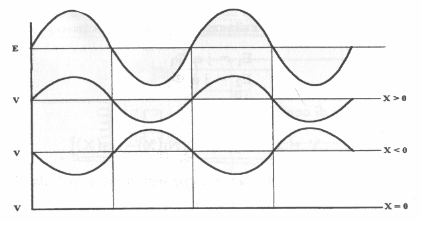
\includegraphics[scale=0.5]
{img/trasformatore-differenziale-fase.png}
	\caption{Segnale in uscita da un trasformatore
differenziale\label{fig:trasdifffase}}
\end{figure}

\section{Trasduttore ad induttanza variabile}

\chapter{Trasduttori di posizione angolare}
\section{Potenziometro circolare}
Il funzionamento è identico a quello di posizione lineare cambia il
fatto che ora si misura un angolo e non una distanza quindi la
relazione ora è la seguente:

	\[V=E\frac{\theta}{360\textdegree}\]

\subsection{Vantaggi}
L'unico vantaggio è la linearità fra la tensione fornita e l'angolo
misurato.
\subsection{Svantaggi}
Gli svantaggi sono, invece, l'ambiguità fra l'inizio e la fine (il
cursore passa da 360 a 0 gradi) e l'esistenza di una zona morta nella
quale non si può misurare per via dell'assenza di contatti.

% \section{Synchro} % FIXME tosto
\section{Encoder binario ed a codice di Gray}
Tramite un encoder è possibile misurare numericamente l'angolo
rilevato, per farlo si utilizza un disco così costituito: tanti
settori quanti sono gli angoli misurabili e tante corone quanti sono i
bit necessari per determinare tutti gli angoli misurabili. Dopo la
divisione alcune aree vengono oscurate per identificare gli zero della
codifica binario o gray. Il codice gray viene utilizzato quando si
vuole eliminare l'ambiguità fra una codifica e l'altra.

\begin{figure}[htbp]
	\centering
	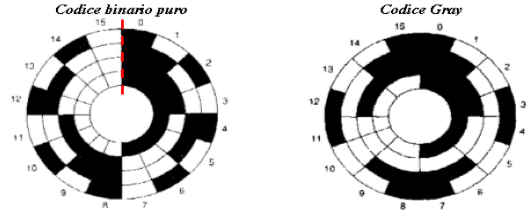
\includegraphics[scale=0.5]
			{img/encoder.png}
	\caption{Encoder binari ed a codice di
Gray\label{fig:encored}}
\end{figure}

Per la rilevazione della codifica vengono usate tante coppie di LED e
foto-transistor quante sono le corone utilizzate; dopo di che, vengono
opportunamente allineati di modo che ogni coppia faccia riferimento
solo ad una corona. Al movimento della corona grazie alle parti scure
è possibile rilevare la codifica dell'angolo.

\section{Encoder incrementale}
Questo tipo di encoder si differenzia dal precedente per l'utilizzo
di solo due corone concentriche suddivise in settori sfasati di un
quarto di periodo.

\begin{figure}[htbp]
	\centering
	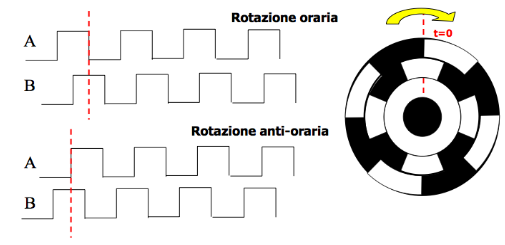
\includegraphics[scale=0.5]
			{img/encoderincr.png}
	\caption{Encoder incrementale\label{fig:encored}}
\end{figure}

In questo modo è possibile riconoscere gli incrementi e i decrementi
di angolo e quindi calcolare l'angolo finale. Indichiamo con $P$ il
fronte positivo e con $N$ il fronte negativo del segnale e con $S_1$
la corona esterna e con $S_2$ la corona interna; ne risulta la
seguente tabella di incrementi:

\begin{center}
\begin{tabular}{lll}
$S_1$ & $S_2$ & incremento\\
P & 0 & +1\\
P & 1 & -1\\
N & 0 & -1\\
N & 1 & +1\\
0 & P & -1\\
1 & P & +1\\
0 & N & +1\\
1 & N & -1
\end{tabular}
\end{center}

A partire dalla posizione di riposo, sarà facile calcolare l'angolo
ottenuto nelle rotazioni.

\chapter{Trasduttori di velocità}
\section{Trasduttore elettromagnetico}
\section{Dinamo tachimetrica}
\section{Alternatori tachimetrici}
\section{Generatori ad induzione}
\section{Trasduttore a carica e scarica capacitiva}
\section{Trasduttore elettro-ottico}
\chapter{Trasduttori di accelerazione}
\section{Accelerometro massa-molla}
Consiste in una scatola in cui è presente una piccola massa che può
muoversi orizzontalmente e che è soggetta ad un'azione di richiamo da
parte di una molla; nello stesso contenitore è presente un trasduttore
di posizione lineare che misura la posizione della massa. Indicando
con $x$ lo spostamento relativo della massa $m$ e applicando le leggi
della fisica per le molle ($k$ costante elastica della molla) possiamo
facilmente ricavare l'accelerazione $a$:

	\[F=ma=-kx \Rightarrow x=-\frac{ma}{k}\]

Data che c'è proporzionalità fra lo spostamento $x$ e l'accelerazione
$a$, possiamo definire la sensibilità del trasduttore come rapporto
fra lo spostamento e l'accelerazione:

	\[x=-\frac{ma}{k} \Rightarrow \frac{x}{a}=-\frac{m}{k}\]

\section{Servo-accelerometro}
Un servo-accelerometro è costituito da una massa $m$ collegata ad un
motore in continua $C$ di modo da far oscillare il rotore del motore.
Quando la massa subisce un'accelerazione questa si sposta e genera
una coppia proporzionale all'accelerazione. Un trasduttore di
posizione lineare rileva lo spostamento della massa rispetto alla sua
posizione di riposo; il segnale in uscita da questo trasduttore è
applicato ad un amplificatore la cui corrente in uscita è applicata
al motore che genera una coppia uguale e contraria a quella fornita
dalla massa. In questo modo la massa ritorna alla sua posizione di
riposto. La tensione misurata sul carico situalo fra il motore e
l'amplificatore ci darà una tensione proporzionale all'accelerazione.

\section{Accelerometro piezoelettrico}
Il principio alla base di un accelerometro piezoelettrico è lo stesso
del massa-molla con l'aggiunta di un cilindretto di materiale
piezoelettrico che assolve le funzioni di richiamo della molla e di
misurazione dello spostamento.
%FIXME trattazione fisica del piezo

\section{Accelerometro MEMS}
Gli accelerometri di questo tipo sono realizzati con tecnologia MEMS
(Micro-Electro-Mechanical-System). Questo tipo di tecnologia permette
di realizzare sensori, attuatori e altri dispositivi elettrinici
mediante un processo di lavorazione di uno strato di silicio.
Un accelerometro di tipo MEMS ha lo stesso principio del massa-molla
ma è realizzato mediante l'uso di gas. All'interno dell'accelerometro
viene creata un piccola bolla di gas riscaldato che si muove in
funzione degli spostamenti. Mediante dei sistemi di misurazione della
temperatura, distribuiti dentro all'accelerometro, è possibile
individuare lo spostamento della bolla quindi ricavare l'accelerazione
che ne ha generato lo spostamento.
\chapter{Trasduttori di temperatura}
\section{Termocoppie e termopile}
Per far si che si possa generare della corrente elettrica le
termocoppie sono costituite da due circuiti metallici di materiale
differente ($M_1$, $M_2$) saldati assieme nei punti dove si
campiona la temperatura di riferimento $T_1$ e la temperatura
da misurare $T_2$.

\begin{figure}[htbp]
	\centering
	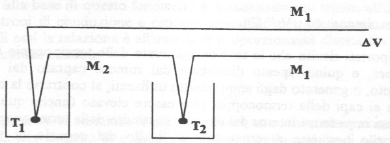
\includegraphics[scale=0.5]
			{img/termocoppia.png}
	\caption{Termocoppia\label{fig:termocoppia}}
\end{figure}

A questo punto se le temperature dove ci sono le saldature sono
differenti si genera della differenza di potenziale $\Delta V$ che
cresce all'aumentare della differenza $T_2-T_1$.
In questo modo possiamo creare una relazione di tipo lineare per
descrivere l'andamento della tensione rispetto alla variazione di
temperatura, invece useremo una relazione non lineare quando la
differenza termica è di qualche decina di °C:

	\[\Delta V = a(T_2 -T_1)\]
	\[\Delta V = a(T_2-T_1)+b(T_2-T_1)^2+c(T_2-T_1)^3+ ...\]

dove i valori di $a$, $b$, $c$ dipendono dai materiali utilizzati.

Un problema delle termocoppie è che la tensione fornita è piccola e
quindi più sensibile al rumore, per questo vengono usate le termopile,
cioè più termocoppie collegate in serie.

\begin{figure}[htbp]
	\centering
	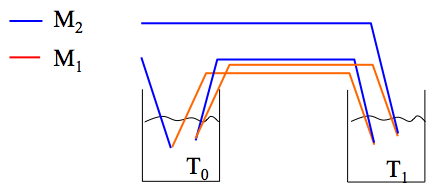
\includegraphics[scale=0.5]
			{img/termopila.png}
	\caption{Termopila\label{fig:termopila}}
\end{figure}

Indicando con $n$ il numero di termocoppie collegate in serie, la
tensione misurata sulla termopila sarà:

	\[\Delta V = na(T_2 -T_1)\]

\section{Termo-resistenze}
Sono resistenze il cui valore cresce con  la temperatura e vengono
spesso indicate dalla  sigl a PTC (Positive Temperature
Coefficient). La relazione  che lega la temperatura assoluta al
valore della resistenza è la seguente:

	\[R=kT_{ass}\]

Volendo però fornire un'approssimazione più realistica introduciamo un
coefficiente alfa, detto coefficiente di temperatura:

	\[\alpha=\frac{1}{R_0}[\frac{dR}{dT}]\]

con R0 e T0 valori di riferimento.

\section{Termistori}
Come le termo-resistenze variano la loro resistività in funzione
della temperatura; sono spesso indicati con la sigla o  NTC (Negative
Temperature Coefficient). La relazione fra la resistività e la
temperatura è la seguente:

	\[R=R_0e^{-D(\frac{1}{T_0}-\frac{1}{T})}\]

dove $R_0$ indica la resistenza di riferimento ad una data
temperatura $T_0$; $B$ è la costante di temperatura

I termistori sono preferibili alle termo-resistenze quando le
variazioni di temperature sono limitate.

\section{Trasduttori integrati di temperatura}
si tratta di circuiti integrati comprendenti una giunzione a
semiconduttore, la cui caratteristica tensione-corrente dipende
fortemente dalla temperatura. La soluzione circuitale più semplice è
rappresentata da due diodi identici alimentati da correnti differenti

\begin{figure}[htbp]
	\centering
	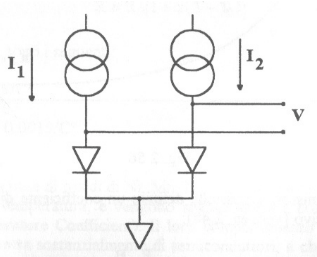
\includegraphics[scale=0.5]
			{img/termointegrati.png}
	\caption{Trasduttori integrati di temperatura
\label{fig:termointegrati}}
\end{figure}


Fissata la corrente entro la giunzione, la caduta di tensione viene
utilizzata come misura della temperatura ed opportunamente
amplificata:

	\[V=\frac{KT}{e}\ln(\frac{I_2}{I_1})\]

questo vale, se e sole se vale la seguente relazione per ogni diodo:

	\[V_d=\frac{KT}{e}\ln(\frac{I_d}{I_0})\]
\chapter{Trasduttori di flusso}
\section{Flussimetro a turbina}
\section{Flussimetro elettromagnetico}
\section{Flussimetro a ultrasuoni}
\section{Venturimetro}
\chapter{Trasduttori di livello}
\section{A galleggiante}
\section{A ultrasuoni}
\section{Resistivo e capacitivo}
\chapter{Estensione}
\section{Trasduttori di deformazione - estensimetri}
Un estensimetro consente di misurare le deformazioni di un oggetto,
di conseguenza può essere usato per misurare una forza applicata, una
coppia o una pressione.
Un estensimetro è costituito da un conduttore metallico filiforme,
sottile, disposto a serpentina su una superficie di supporto. La
superficie di supporto può essere in carta alla nitrocellulosa, in
resina epossidica, fibra di vetro.

%\begin{figure}[htbp]
%	\centering
%	\includegraphics[scale=0.5]
%			{img/estensimetro.png}
%	\caption{Estensimetro\label{fig:estensimetro}}
%\end{figure}

Il supporto viene incollato all'oggetto di cui si vuole misurare la
deformazione. La sensibilità è espressa tramite il gage-factor $g$
cioè come il rapporto fra la variazione relativa della resistenza e la
variazione relativa della lunghezza:

	\[g=\frac{\frac{\Delta R}{R}}{\frac{\Delta L}{L}}\]

Si osserva che il valore della resistenza varia quando questa è
deformata secondo la legge:

	\[R=\rho\frac{L}{S} \Rightarrow L =\frac{RS}{\rho}\]

dove con $\rho$ indichiamo la resistività, con $L$ la lunghezza del
resistore e con $S$ la sua sezione.
Il conduttore filiforme è disposto a serpentina di modo da essere
molto sensibile alle deformazioni nella direzione della serpentina e
poco sensibile altrimenti. Per effetto della deformazione otteniamo:

	\[dR=\rho\frac{dL}{S} + d\rho\frac{L}{S} -
	     \rho\frac{L}{S^2}dS\]

da cui:

	\[g=\frac{LdR}{RdL}=\frac{\rho L}{SR}+
			    \frac{L^2}{SR}\frac{d\rho}{dL}-
			    \frac{L^2\rho}{S^2dLR}dS
	   =1+\frac{Ld\rho}{\rho dL} - \frac{L dS}{S dL}\]

Ricordando che un materiale sotto sforzo non modifica il proprio
volume

%FIXME altri conti che non sono chiari

%FIXME cos'era sta roba?
%La temperatura può essere influente sul valore della resistenza così
%per compensare questo disturbo si utilizzano due estensimetri con
%lavoro opposto: uno misura l'estensione, l'altro la compressione. Per
%misurare ora il valore della tensione associato alla deformazione
%utilizziamo il partitore di tensione fra i due estensimetri le cui
%resistenze valgono:

%Dove $R_1$ è per l'estensione, $R_2$ per la compressione, $R_0$
%valore a riposo della resistenza e ∆R(t) la variazione dovuta alla
%temperatura.

Gli estensimetri possono essere utilizzati anche per misurare la forza
conoscendo la deformazione di un pezzo campione, dal modulo di
elasticità e dalla sezione trasversale del provino; si può anche
misurare la coppia rilevando la deformazione di un albero mediante due
estensimetri messi a croce con inclinazione a 45° rispetto all'albero,
in questo modo un estensimetro risulta compresso e uno esteso; infine
si possono utilizzare per misurare la pressione, ma in questo caso si
utilizzano estensimetri a forma di fiore di modo che possano misurare
in ogni direzione.

\section{Trasduttori di pressione}
I più comuni sono costituiti da una membrana e da diaframmi i quali
subiscono una deformazione per effetto della pressione applicata, si
andrà poi a misurare questa deformazione con un estensimetro e quindi
convertita in grandezza elettrica. Altri tipi utilizzati sono quelli a
soffietto o a tubo di Bourdon.

\begin{figure}[htbp]
	\centering
	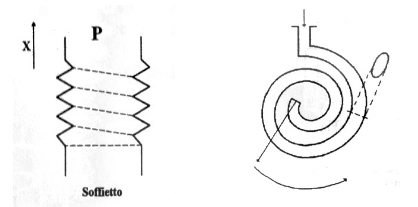
\includegraphics[scale=0.5]
			{img/pressione.png}
	\caption{Trasduttori di pressione
\label{fig:pressione}}
\end{figure}

Con il soffietto si misurano gli spostamenti, quindi si utilizzerà un
trasduttore di posizione per rilevare la pressione; il tubo di Bourdon
è costituito da un tubo a sezione ellittica avvolto a spirale alla cui
estremità è attaccato un ago: applicando la pressione sulla parte
esterna genera una rotazione dell'ago proporzionale alla pressione
imposta, andremo quindi a misurare un angolo.
I trasduttori a membrana sono utilizzati per le misure grandi, i due
tipi appena descritti, invece, per le piccole misurazioni.
\section{Trasduttori di livello - livellometri}
\chapter{Attuatori}
\section{Motori in corrente continua}
In questo tipo di motori, la coppia applicata all'albero è
proporzionale alla corrente circolante negli avvolgimenti del motore
$\Gamma = KI$. Inoltre la tensione ai capi del motore risulta
proporzionale alla velocità del motore; questo vale sotto l'ipotesi di
rendimento massimo, ovvero senza perdite di energia, ne consegue che
$V=K\omega$. Da queste considerazioni ne consegue che
$\Gamma\omega=VI$

\section{Motori passo-passo}
I motori passo-passo sono motori comandati da segnali logici. Questo
ha il vantaggio della perfetta riproduzione dei movimenti e della
capacità di mantenere la posizione raggiunta. Il motore si basa fra
l'accoppiamento di un ingranaggio di materiale ferromagnetico e di 4
avvolgimenti statorici contigui. Gli avvolgimenti vengono posti ad
una distanza di un angolo pari ad $\frac{1}{4}$ dell'angolo fra due
denti dell'ingranaggio.

Gli avvolgimenti sono alimentati due alla volta in ordine
sequenziale, questo muove l'ingranaggio. Il dente dell'ingranaggio
allineato al primo avvolgimento viene attratto dai successivi man
mano che questi vengono alimentati, questo produce la rotazione
dell'ingranaggio. Al termine della rotazione, il dente successivo
viene attratto dagli avvolgimenti.

\section{Attuatore elettromagnetico}
Questo tipo di attuatore è realizzato come il trasduttore di velocità
lineare. Una barretta magnetizzata è posta parzialmente all'intero di
un solenoide. Nel momento in cui il solenoide viene alimentato, la
berretta subisce una forza di attrazione o repulsione dal solenoide
che è proporzionale alla corrente che scorre nel solenoide. Sia $v$ la
velocità con cui si sposta il magnete, $n$ il numero di spire, $V$ la
tensione ai capi del solenoide e $I$ la corrente che vi scorre;
possiamo calcolare la forza applicata:

	\[V=n\phi_Bv, VI=Fv\]
	\[F= \frac{VI}{v}=n\phi_B I\]
\chapter{Reti di condizionamento}

\part{Controlli}
\chapter{Algoritmi di controllo}
\section{Introduzione}
\section{Controllo ON-OFF}
Si tratta di un tipo di controllo molto semplice che in cui gli
attuatori o si accendono o si spengono.
\section{Controllo proporzionale}
Il principio alla base di questo tipo di controllo è l'errore fra la
variabile misurata e il suo valore atteso; di conseguenza l'attuatore
viene regolato di modo da muovere il sistema vero il valore atteso.
\section{Controllo integrale}
\section{PID}
\section{Feed-Forward}
Quando si conoscono in anticipo le evoluzioni del sistem è possibile
agire sull'attuatore prima che si verifichino di modo da compensarne
gli effetti.
\section{Controllo mediante calcolatore}
Se variabili di controllo vengono campionate ed analizzate da un
calcolatore.

Mediante calcolatore è possibile implementare anche gli algoritmi di
controllo classici.

\end{document}
